\chapter{Цель и задачи}
\label{ch:intro}

\textbf{Цель}: Изучение методов создания и анализа цепей Маркова \\

\section*{Задание к лабораторной работе}

\begin{figure}[H]
    \centering
    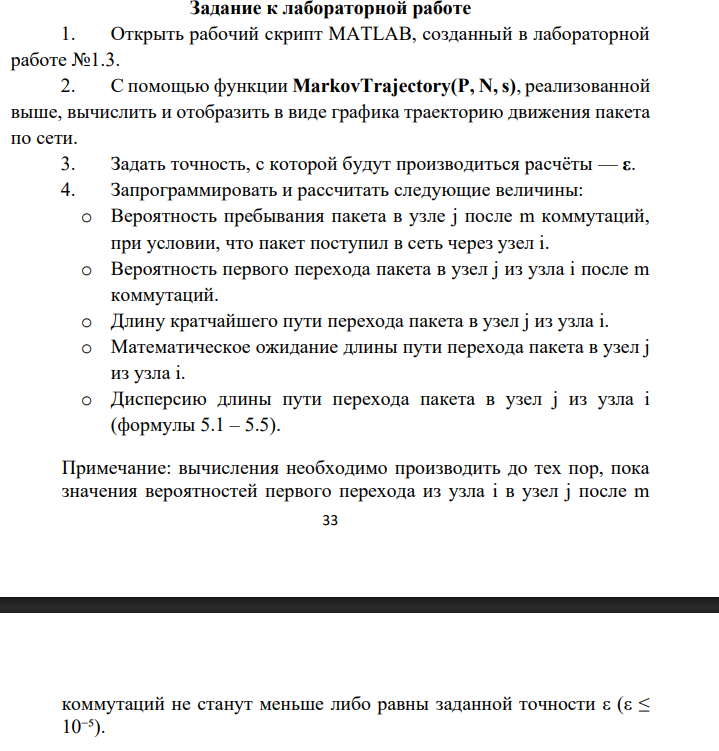
\includegraphics[width=1.0\textwidth]{task1.png}
    \caption{Задание для лабораторной работы}
\end{figure}

\begin{figure}[H]
    \centering
    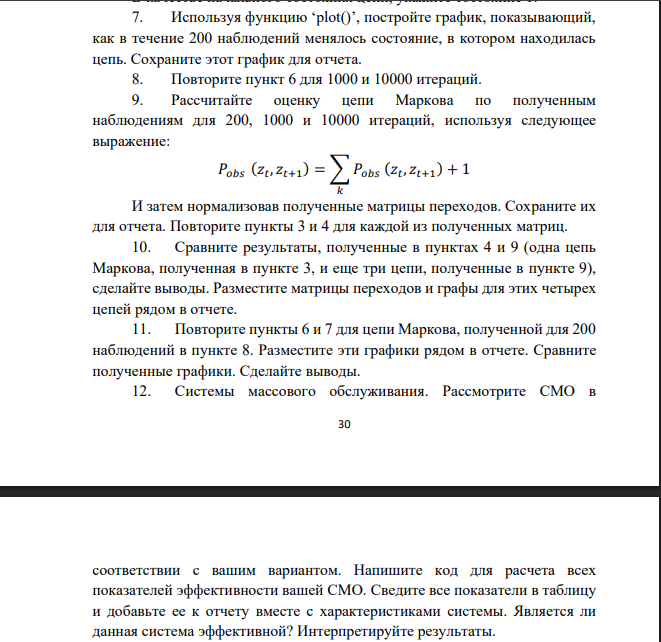
\includegraphics[width=1.0\textwidth]{task2.png}
    \caption{Задание для лабораторной работы}
\end{figure}

\begin{figure}[H] 
    \centering
    
\includegraphics[width=1.0\textwidth]{task3.png}
    \caption{Задание для лабораторной работы}
\end{figure}

\begin{figure}[H]
    \centering
    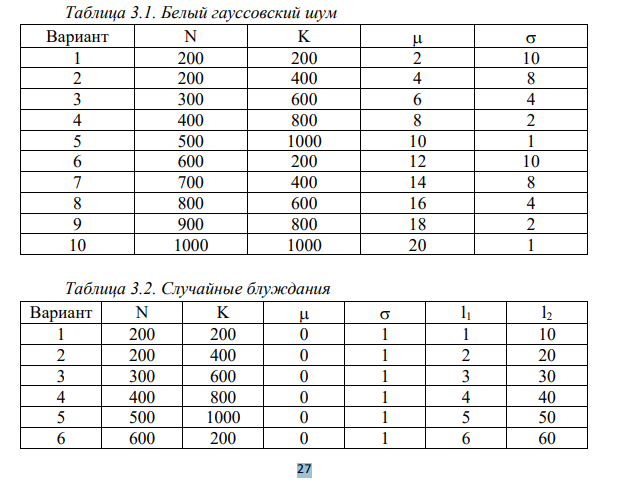
\includegraphics[width=1.0\textwidth]{tables.png}
    \caption{Варианты заданий}
\end{figure}



\endinput